\documentclass{article}


\newlength\tindent
\setlength{\tindent}{\parindent}
\setlength{\parindent}{0pt}
\renewcommand{\indent}{\hspace*{\tindent}}

\usepackage[left=2.5cm,top=3cm,right=2.5cm,bottom=3cm,bindingoffset=0.5cm]{geometry}
\usepackage{amssymb} % For \mathbb
\usepackage{amsmath}
\usepackage{xcolor}
\usepackage{array} % for better column definitions
\usepackage{booktabs} % for better table lines
\usepackage{caption} % for captioning tables
\usepackage{cancel}
\usepackage{tikz}
\usetikzlibrary{arrows.meta, graphs, positioning} % Load necessary TikZ libraries
\newcommand{\negation}{${\phantom{0}}^\sim$}
\newcommand{\theorum}[1]{\quad \quad \colorbox{yellow}{\textit{\textcolor{red}{Theorum #1}}}}
\newcommand{\sub}[1]{\vspace{10pt}\textbf{#1}}
\newcommand{\sbreak}{\vspace{10pt}}

\title{CS1231S Note}
\begin{document}

\maketitle

\section{Speaking Mathematically}

\subsection{Defintions}

\begin{tabular}{rl}
    Natural Numbers\quad & $\mathbb{N}$ = \{ 0, 1, 2, 3, ... \} \\
    Integers\quad & $\mathbb{Z}$ = \{ -100, 3, 21, 32, ... \} \\
    Rational Numbers\quad & $\mathbb{Q}$ = \{ -23, 8.6, $\frac{1}{2}$, 3, ... \}\\
    Real Numbers\quad & $\mathbb{R}$ = \{ -1, $\pi$, $\sqrt{2}$, 4.5, ...   \}
\end{tabular}

\subsubsection{Real Numbers vs Rational?}
Rational numbers ($\mathbb{Q}$) are numbers that can be represented as a ratio of two numbers, e.g. $\frac{4}{3}$. Real numbers ($\mathbb{R}$) is the set of rational \& irrational numbers.

\subsection[Properties of Integers]{Properties of Integers\footnote{1.3.3 pg.26}}
\begin{itemize}
    \item Closure \quad \textcolor{red}{$x + y \in \mathbb{Z}$}
    \item Commutativity \quad \textcolor{red}{$x + y = y + x$}, and, \textcolor{red}{$xy = yx$}
    \item Associativity \quad \textcolor{red}{$x + y + z = (x + y) + z = x + (y + z)$}, and \textcolor{red}{$xyz=(xy)z=x(yz)$}
    \item Distributivity \quad \textcolor{red}{$x(y+z) = xy + xz$}
    \item Trichotomy \quad \textcolor{red}{$x = y$}, or, \textcolor{red}{$x < y$}, or \textcolor{red}{$x > y$}
\end{itemize}


\subsection[Even and Odd Integers]{Even and Odd Integers\footnote{1.3.4 pg.27}}
\quad n is even $\Leftrightarrow \exists k$ s.t. $n = 2k$

\quad n is odd $\Leftrightarrow \exists k$ s.t. $n = 2k+1$

\subsection{Proofs in Lecture 1}
\begin{itemize}
    \item Product of two consecutive odd numbers is always odd\footnote{1.3.4 pg. 28}
\end{itemize}

% LECTURE 2 Propositional Logic ==================================
\section{Propositional Logic}
\subsection{Definitions}
\subsubsection{Statements}
A statement is a sentence that is true or false, but not both.
\subsubsection{Negation}
If p is a statement variable, the negation of p is "not p", denoted \textcolor{red}{\negation p}
\subsubsection{Conjunction}
Conjunction of 2 statement variables p, q, said "p and q", is denoted \textcolor{red}{p $\wedge$ q}
\subsubsection{Disjunction}
Disjunction of 2 statement variables p, q, said "p or q", is denoted \textcolor{red}{p $\vee$ q}
\subsubsection{Statement Form}
A statement form is an expression made up of statement variables and logical connectives
\subsubsection{Logical Equivalence}
Two statements are logically equivalent iff they have identical truth values. Denoted \textcolor{red}{p $\equiv$ q}
\subsubsection{Tautology}
A statement form that is \textcolor{red}{always true}
\subsubsection{Contradiction}
A statement form that is \textcolor{red}{always false}
\subsubsection{Conditional (only if)}
Given statement variables p and q, "if p then q", or "p implies q" is denoted \mbox{\textcolor{red}{p $\rightarrow$ q}}. p is the antecedent, and q is the consequent.

In this example, p is a \textcolor{red}{sufficient condition} for q - the "existence" of p guarantees the "existence" of q

q is a \textcolor{red}{neccessary condition} for p - if q occurs, p \textit{may} occur.

\sbreak
\begin{center}
    $p\rightarrow q$ $\equiv$ \negation$p \vee q$
\end{center}

\subsubsection{Converse, Inverse, Contrapositive}
Given a statement P$\rightarrow$Q,

1. \textbf{Converse}:
Q$ \rightarrow$ P

2. \textbf{Inverse}:
\negation P$\rightarrow$ \negation Q

Converse $\equiv$ Inverse

\vspace{10pt}

3. \textbf{Contrapositive}:
\negation Q $\rightarrow$ \negation P

Contrapositive $\equiv$ Original Statement


\subsubsection{Vacuous Truth}
A conditional statement that is true by virtue of the fact that its hypothesis is false
\subsubsection{Biconditional}
Given stmt variables p and q, "p, if and only if, q" is denoted \textcolor{red}{p$\leftrightarrow$q}

p is a \textcolor{red}{necessary and sufficient} condition for q

\subsection{Truth Table of Operators}
\begin{tabular}{|c|c|c|c|c|c|}
    \hline
    P & Q & P$\vee$Q & P$\wedge$Q & P$\rightarrow$Q & P$\Leftrightarrow$Q \\
    \hline
    T & T & T & T & T & T  \\
    T & F & T & \textcolor{red}{F} & \textcolor{red}{F} & \textcolor{red}{F}  \\
    F & T & T & \textcolor{red}{F} & T & \textcolor{red}{F}  \\
    F & F & \textcolor{red}{F} & \textcolor{red}{F} & T & T  \\
    \hline
\end{tabular}


\subsection{Order of operation of statements}
First

\begin{tabular}{|c|c|}
    \hline
    Op1 & Op2 \\
    \hline
    \textbf{$\sim$} &  \\
    $\wedge$  & $\vee$  \\
    $\to$ & $\iff$  \\
    \hline
\end{tabular}

Last

\subsection{Arguments}
Arguments are a sequence of statements. All statements except the final one are called \textbf{premises}

\vspace{10pt}

if p, then Q \quad\quad $\leftarrow$  premise

p\quad\quad\quad\quad\quad\quad\quad $\leftarrow$  premise

therefore q \quad\quad $\leftarrow$ conclusion

\subsubsection{Modus Ponens}
p $\rightarrow$ q

p

•q

\subsubsection{Modus Tollens}

p $\rightarrow$ q

\negation q

•\negation p

\subsubsection{Generalization}

p

•p $\vee$ q

\vspace{10pt}

q 

•p $\vee$ q

\subsubsection{Specialization}

p$\wedge$q

•p

\vspace{10pt}

p$\wedge$q

•q

\subsubsection{Transitivity}
p$\rightarrow$q

q$\rightarrow$r

•p$\rightarrow$r

\subsubsection{Proof By Division into Cases}
p$\vee$q

p$\rightarrow$r

q$\rightarrow$r

•r

\subsubsection{Contradiciton Rule}

\negation p$\rightarrow$false

•p

\subsubsection{Fallacies}
\textbf{1. Converse Error}

p$\rightarrow$q

q

•p

\vspace{10pt}
\textbf{2. Inverse Error}

p$\rightarrow$q

\negation p

•\negation q

\vspace{10pt}
\textbf{3. False Premise}

When the premise is not true, e.g. If you're Singaporean, then you're rich.

\subsubsection{Checking the Validity of Arguments}
To do this, construct a truth table and then check the \textcolor{red}{critical rows}. Critical rows are rows in which each premise evaluates to \textcolor{blue}{true}. If the conclusions are also true in the critical rows, they are valid.

Now consider that a premise with contraditions will have no critical rows. This makes it vacuously valid.

\section{Predicate Logic}
\subsection{Definitions}
\subsubsection{Predicate}
A predicate is a sentence that contains a finite number of variables and becomes a statement when specific values are substituted for the variables.
The domain is the set of all values that may be subbed in place of the variables.
\subsubsection{Truth Set}
The set of all elements of domain D that make P(x) true, denoted 
\{x$\in$D $\mid$ P(x)\}
\subsubsection{Universal Statement}
A universal statement of the form $\forall$x$\in$D, Q(x) is defined to be true iff Q(x) is true for all x in D. It is false if Q(x) is \textcolor{red}{false for at least one of x in D}.
\subsubsection{Existential Statement}
A existential statement of the form $\exists$x$\in$D, Q(x) is defined to be true iff Q(x) is true for at least one x in D. It is false iff Q(x) is false \textcolor{red}{for all x in D}
\subsubsection{Existential Quantifier}
The symbol $\exists$! denotes "There exists a unique".
\subsubsection{Negation of Universal Statements}
A universal statement $\forall$x$\in$D, Q(x) is negated like so:
$\exists$x$\in$D, \negation Q(x) \theorum{3.2.1}
\subsubsection{Negation of Existential Statements}
An existential statement $\exists$x$\in$D, Q(x) is negated like so:
$\forall$x$\in$D, \negation Q(x) \theorum{3.2.2}
\subsubsection{Universal Instantation}
If some property is true of everything in the set, then it is true of any particular thing in the set.

Universal instantation is taking an instance of something in that set, and using the properties on the set to prove some particular thing.
\subsubsection{Universal Generalization}
Paraphrased from tutorial: It is using an extablished property for an arbitrarily chosen element in the domain, and generalizing it to the domain as a whole.

\subsection{Lessons Learnt}
\subsubsection{Complicated Quantifiers}
The order of quantifiers matter. $\forall$ x $\exists$ y means "For all x there exists a y" - the y is variable across x.

$\exists$ x $\forall$ y means "There exists a x for all y" - the x is \textbf{fixed} for all values of y.

\vspace{10pt}

When there are multiple existential qualifiers, things can get confusing but try to "scope" it.
e.g. \begin{math}
    \forall x \exists y \forall z
\end{math} - Scope the first two terms. The y is variable across x. Then, the last two terms - a specific y must work for all z.
\subsubsection{Always consider the counterexample when proving an implication}
If you see an implication, immediately consider the counterexample where T $\rightarrow$ F

\subsubsection{Consider all sides in counterexamples}
Just don't be careless. e.g. $\forall x, y \in \mathbb{Q}, (x\neq y \rightarrow \exists m \in \mathbb{Q}((x<m)\wedge(m<y)))$. Considered that it's possible that in a real number line there's always a number between 2 other numbers - but is it always more than x and less than y? Nope!

\subsubsection{Universal statements apply for all, unless Implication}
Consider the distinction between $\forall x \in A\ ({P(x) \wedge Q(x)})$ and $\forall x \in A\ ({P(x) \rightarrow Q(x)})$. The first statement states that P(x) and Q(x) are true for all x. The second statement has an \textit{if}. Simple but don't get careless.

% LECTURE 5 Set Theory ==================================
\section{Set Theory}

\subsection{Definitions}
\subsubsection{Sets}
Sets are an \textcolor{red}{unordered} collection of objects. The objects are members of sets

Membership of sets is denoted x$\in$S

The cardinality of the set, denoted $\mid$S$\mid$, is the amount of elements in the set.

\subsubsection{Set Notations}
\textbf{1. Set Roster Notation}

Specifies all members of the set.

S = \{1, 2, 3\}

\vspace{10pt}

\textbf{2. Set Builder Notation}

Builds a set using a predicate.

S = \{x$\in$U : P(x)\}

e.g. S = \{(x,y) $\in \mathbb{Z} \times \mathbb{Z}:$ x=2z for some $Z \in \mathbb{Z}$ \}

This builds a set for ordered pairs where x must be even and y is \textbf{unrestricted}

\vspace{10pt}

\textbf{3. Set Replacement Notation}

Similar to Set builder, but reversed

S = \{t(x) : x$\in$U\}

\vspace{10pt}
\textbf{4. Interval Notation}

Describes a set using mathematical equalities.

(a, b) = \{x$\in \mathbb{R}$: a $<$ x $<$ b\}

\subsubsection{Definition of Subset}
A is a subset of B iff every element of A is also an element of B.

\begin{center}
    A $\subseteq$ B iff $\forall$x$\in$A$\rightarrow$x$\in$B
\end{center}

\vspace{10pt}

\textbf{A note on subsets}.
Ensure the comparison of items are always in the same "scope".
e.g. if A = \{1, 2, 3\} and B = \{ \{1,2,3\}, 4, 5, 6\}, then A$\in$B, but A$\nsubseteq$B

\subsubsection{Proper Subsets}
A is a proper subset of B iff A is a subset of B \textbf{and} A$\neq$B.

Denoted A$\subsetneq$B.

\subsubsection{Set equality}
If A$\subseteq$B and B$\subseteq$A, then A=B.

\subsubsection{Set difference}
The difference of B minus A, denoted B\textbackslash A, is the set of all elements that are in B and not A.

Symbolically,
\begin{center}
    $B$\textbackslash $A = \{ x \in U : x \in B \wedge x \notin A \}$
\end{center}

\vspace{10pt}

\textbf{A note on set difference}.

Again, always consider the scope. If A = \{1,2,3,\{4\}\} and B = \{4\}, then \mbox{A\textbackslash B = \{1,2,3,\{4\}\}}

\textbf{Another note.} Any set differenced by the empty set is the set itself.

\subsubsection{Union of Sets}
A union of 2 sets is the set of all elements in either set.

Symbolically,
\begin{center}
    $A\cup B = \{ x \in U: x\in A \vee x\in B\}$
\end{center}

\subsubsection{Intersection of Sets}
An intersection of 2 sets is the set of all elements appearing in \textbf{BOTH} sets.

Symbolically:
\begin{center}
    $A\cap B = \{ x\in U: x\in A \wedge x \in B\}$
\end{center}

\subsubsection{Complement of Sets}
The complement of a set A is all the elements in the domain that are not in A.

Symbolically,
\begin{center}
    $\bar{A}$ = \{ x $\in$ U $\mid$ x$\notin$A\}
\end{center}

\subsubsection{Empty Sets}
A set with no element is denoted $\varnothing$.

An empty set is a subset of every set. $\varnothing \subseteq \forall A$ \theorum{6.2.4}

\subsubsection{Ordered Pairs}
An ordered pair is of the form (x,y)

\sub{Equality of ordered pairs}

Two ordered pairs (a,b) and (c,d) are equal iff \break a=c $\wedge$ b=d. \textbf{Remember} to explicitly show and write this out in proofs.

\subsubsection{Cartesian Products}
The cartesian products of two sets A and B is the set of all ordered pairs (a,b) where a$\in$A and b$\in$B.

Symbolically,
\begin{center}
    $A \times B = \{ (a,b)\ :\ a\in A \wedge b \in B\}$
\end{center}

\sbreak

Cardinality of cartesian product is $\mid A\mid \times \mid B\mid$

\subsubsection{Mutually Disjoint Sets}
Two sets are disjoint iff A$\cap$B = $\varnothing$

Multiple Sets A1,A2,...An are \textbf{mutually disjoint} if no two sets Ai and Aj have any elements in common.

\subsubsection{Partitions of Sets}
A division of sets into \textcolor{red}{mutually disjoint} sets.

\subsubsection{Power Sets}
Given a set A, the \textbf{power set} of A is the set of all subsets of A.

Symbolically,
\begin{center}
    $ x \in \mathcal{P}(A) \iff x \subseteq A $
\end{center}

\vspace{10pt}

\textbf{Power sets of empty set}

$\mathcal{P}$($\varnothing$) = \{ $\varnothing$ \}

The power set of an empty set is the set containing the empty set - the empty set is the subset of every set.

The $\mathcal{P}(\mathcal{P}(\varnothing))$ = \{ $\varnothing$, \{ $\varnothing$ \} \}

Always consider how the set at hand can be rearranged into subsets. If things get confusing, verify with cardinality - $\mid \mathcal{P}(A) \mid = 2^{\mid A \mid}$

\vspace{10pt}

\textbf{Cardinality of power set}

The cardniality of any power set is given $2^n$ where n = $\mid A \mid$

\subsection{Lessons Learnt}
\subsubsection{Union of Power Sets}
$\mathcal{P}(A \cup B) \neq \mathcal{P}(A) \cup \mathcal{P}(B)$. Think of the biggest set in $A \cup B$ - the set of the elements in \textit{both} A and B is not included in the union of two power sets.

\subsubsection[Intersection of Power Sets]{Intersection of Power Sets \footnote{Assignment 1 Qn 6c}}
$\mathcal{P}(A \cap B) = \mathcal{P}(A) \cap \mathcal{P}(B)$.

\subsubsection{Difference of empty set}
Any set S\textbackslash$\varnothing$ = S.
Empty set has no elements, so elements in S that are not in the empty set is S.

\subsubsection{Empty set confusion}
Sometimes, empty sets can get confusing. When dealing with intersections or unions, I prefer to "enumerate" the empty set. That is, instead of using $\varnothing$, use \{\}. As such, it can be seen that any set A $\cap\ \{\} = \varnothing$

\subsubsection{Properties of Sets}
For all sets A, B, and C, 

\vspace{10pt}

\textbf{Inclusion of Intersection} \theorum{6.2.1}

a)  $A \cap B \subseteq A$

b) $A \cap B \subseteq B$

\vspace{10pt}

\textbf{Inclusion in Union}

a) $A \subseteq A \cup B$

b) $B \subseteq A \cup B$

\vspace{10pt}

\textbf{Transitive property of subsets}

$A \subseteq B \wedge B \subseteq C \rightarrow A \subseteq C$

\sub{Using properties for proofs}

Make sure that you're strictly following these properties in proofs. E.g. if $S \subseteq A\cap B$, you cannot simply state $S \subseteq A$. Use the properties like so:
\begin{center}
    $A \cap B \subseteq A$ (Inclusion of Intersection)\\
    $S \subseteq (A \cap B) \wedge (A \cap B) \subseteq A$\\
    $S \subseteq A$ (Transitive property of subsets)
\end{center}

% LECTURE 6 RELATIONS ==================================
\section{Relations}
\subsection{Definitions}
\subsubsection{Relation}
A relation from A to B is a subset of $A\times B$

Given an ordered pair (x,y) in $A\times B$, $xRy$ iff (x,y) $\in$ R.

\subsubsection{Domain, Co-domain, Range}
\textbf{Domain} is the set $\{ a \in A :\ aRb\ for\ some\ b \in B\}$

\vspace{10pt}

\textbf{Co-domain} is the set B.

\vspace{10pt}

\textbf{Range} is the set $\{b \in B :\ aRb\ for\ some\ a\ \in A\}$

\subsubsection{Inverse Relations}
If R is a relation from A to B, the inverse relation $R^{-1}$ is from B to A as follows:
$R^{-1} = \{(y,x) \in B \times A : (x,y) \in R\}$

\subsubsection{Composition of Relations}
Let A, B, and C be sets. Let $R \subseteq A \times B$ be a relation, and $S \subseteq B \times C$ be a relation. The \textbf{composition of R with S}, denoted $S \circ R$ is the relation from A to C such that:

\vspace{10pt}

$\forall x \in A, \forall z \in C\ (x S \circ R z \iff (\exists y \in B (xRy \wedge ySz)))$

\vspace{10pt}

In other words, there must be some "link" (y in the above) between the two Relations

\vspace{10pt}

To find $R \circ R \circ ... \circ R$, we can put R in a graph first. Count how many R's there are - this is the amount of compositions. Then, check the graph for walks of count(R) - put in adjacency matrix

\textbf{Composition of Self-Relations}

A relation can be composited by itself. (From tutorial) In a digraph, an easy way to compute $R \circ R$ is as follows. (i) Start with the first element $a$ and trace all possible destinations after taking exactly $n$ arrows, $n$ being the amount of compositions + 1. So if $R \circ R$, n=2. (ii) In a separate graph, draw the arrows pointing from the start element to the end. (iii) Repeat for all other elements.

\vspace{10pt}

\textbf{Associativity of Compositions}

$T \circ (S \circ R) = (T \circ S) \circ R = T \circ S \circ R$

\textcolor{red}{Do not confuse this for commutativity! Compositions are noncommutative.}

\vspace{10pt}

\textbf{Inverse of Compositions}

$(S \circ R)^{-1} = R^{-1} \circ S^{-1}$

\subsubsection{Reflexivity}
R is reflexive iff $\forall x \in A\ (xRx)$

\vspace{10pt}

Note that this is not an implication, and thus cannot be vacuously true. That is to say, every element in the domain of the relation (in this case, A) MUST have a self-relation to be considered reflexive.

\subsubsection{Irreflexivity}
R is irreflexive iff $\forall x \in A\ (x\cancel{R}x)$
\subsubsection{Symmetry}
R is symmetric iff $\forall x,y \in A\ (xRy \rightarrow yRx)$

\vspace{10pt}

Note that this \textit{\textbf{is}} an implication, and thus \textit{can} be vacuously true if there is no xRy.


\subsubsection[Asymmetry]{Asymmetry\footnote{Tutorial 5 Qn. 8}}
It's worth noting that asymmetry $\neq$\negation symmetry.

$\forall a,b \in A (aRb \rightarrow b\cancel{R} a)$

\subsubsection{Antisymmetry}
\begin{center}
    $\forall x,y \in A\ (xRy \wedge yRx \rightarrow x=y)$
\end{center}

\subsubsection{Transitivity}
R is transitive iff $\forall x,y,z \in A\ (xRy \wedge yRz \rightarrow xRz)$

Same as above, this can be vacuously true.

\vspace{10pt}

\textbf{Exhaustively checking transitivity}

To exhaustively check transitivity of a relation with N amount of elements, you'd have to check every triplet that fulfils $aRb, bRc, aRc$. In a set with N elements, there are $N^2$ amount of possible pairs, because each element is related to N other elements, including itself. Now, for each pair (a,b), we need to check all (b,c) pairs. There are N (b,c) pairs, as b is related to n c's. So, Each pair in the set is compared with N other pairs, so $\mathbf{N^3}$ checks are needed.

\subsubsection{Transitive Closure}
The transitive closure of a relation R fulfills these 3 properties

1. $R^t$ is transitive

2. $R \subseteq R^t$

3. If S is any other transitive relation that contains R, then $R^t \subseteq S$

\vspace{10pt}

That is to say, the transitive closure is the \textit{smallest} set that makes the relation R transitive.

\subsubsection{Parititions (again)}
$\mathcal{C}$ is a partition of set A if the following hold:

1) $\mathcal{C}$ is a set for wihch all elements are non-empty subsets of A.

2) Every element of A is in exactly one element of $\mathcal{C}$

Elements of a partition are called components of the partition.

Symbolically,
\begin{center}
    $\forall x \in A, \exists!S\in\mathcal{C}\ (x \in S)$
\end{center}

\subsubsection{Relation induced by partitions}
Given a partition $\mathcal{C}$ on a set A, the relation R \textbf{induced by the partition} is defined on A as follows:
\begin{center}
    $\forall x,y, \in A,$
    
    $xRy \iff \exists\ a\ component\ S\ of\ \mathcal{C}\ s.t.\ x,y \in S$
    
\end{center}

A relation induced in this manner is reflexive, symmetric, and transitive. \theorum{8.3.1}

\subsubsection{Equivalence Relations}
An equivalence relation is a relation R that is \textbf{reflexive, symmetric, and transitive}. The symbol $\sim$ denotes an equivalence relation. Additionally, the relation should partition the domain into dijoint sets, so each element must reside in 1 and only 1 equivalence class.

\subsubsection{Equivalence Classes}
The equivalence class of $a$, denoted [a], is the set of all elements x $\in$ A s.t. a is ~ related to x.

Symbolically,
$[a]~ \equiv \{ x \in A:\ a \sim x \}$

\vspace{10pt}

\textbf{A note on listing equivalent classes}

Note that the equivalence class of a relation refers to the \textit{elements} of the set A. While the relation are ordered pairs (x,y), [x] = \{x, y\}. The equivalence class is not an ordered pair.

\subsubsection{Partition Induced by an Equivalence Relation}
If A is a set and R is an equivalence relation on A, then the distinct equivalence classes of R form a partition of A. \theorum{8.3.4}

Essentially saying, the equivalence classes are nonoverlapping.

\subsubsection{Dividing a set by an equivalence relation}
$A/\sim$ is the set of all equivalence classes with respect to $\sim$

$A/\sim = \{ [x]\sim:\ x \in A \}$

e.g. S = \{ 1, 2, 3, 4, 5, 6\}. Then, we have some $\sim$ s.t. [1] = \{1,2\}, [3] = \{3,4,5,6\}.

Then, $A/\sim$ = \{ \{1,2\}, \{3,4,5,6\}\}

\subsubsection{Antisymmetry}
R is antisymmetric iff

\begin{center}
    $\forall x,y \in A\ (xRy\wedge yRx \rightarrow x=y)$
\end{center}

It's negation, R is \textbf{not antisymmetric} iff
\begin{center}
    $\exists x,y \in A (xRy \wedge yRx \wedge x\neq y)$
\end{center}

\vspace{10pt}

\textbf{Antisymmetry and not symmetric are different}

Observe carefully. Antisymmetry and symmetry can happen at the same time: think xRx.

\subsubsection{Partial Order Relations}
R is a \textbf{partial order relation} iff 

1. R is reflexive

2. R is antisymmetric

3. R is transitive

\vspace{10pt}

A partial order of two elements x and y is denoted $x \preccurlyeq y$, where x occures \textit{before} y. I prefer to call it x "unlocks" y.

\vspace{10pt}

\textbf{Can a relation be a partial order and equivalence relation at the same time?}

This essentially asks if a relation can be reflexive, antisymmetric, symmetric, and transitive at the same time. The only case in which asymmetry and symmetry holds is if there are no distinct x and y s.t. xRy. So they're all self-relations.

\subsubsection{Comparability}
\textbf{Elements} in a partial order are comparable if either $a \preccurlyeq b$ or $b \preccurlyeq a$. Otherwise, they are noncomparable.

\vspace{10pt}

A \textbf{set} is comparable iff
\begin{center}
    $\forall x,y \in A\ (xRy\vee yRx)$
\end{center}

Note that this is not an implication - all elements \textbf{have} to be related in one way with another!

In a Hasse Diagram, an element is comparable with all elements in any chain containing that element.

\subsubsection[Compatibility]{Compatibility \footnote{Tutorial 5, Qn. 9}}
Two elements a and b are \textbf{compatible} iff there exist some c $\in$ A s.t. $a \preccurlyeq c$ and $b \preccurlyeq c$

\subsubsection{Maximal, Minimal, Largest, Smallest Elements}
\textbf{Maximal Elements}

Symbolically, $\forall x \in A (c\preccurlyeq x \rightarrow c=x)$

Essentially, if c is "unlocks" an element x, it must be itself. Note the implication, which means noncomparable elements do not prevent a c from being a maximal element

\vspace{10pt}

\textbf{Minimal Elements}

$\forall x \in A (x \preccurlyeq c \rightarrow c=x)$

If any element "unlocks" c, it must be itself.

\vspace{10pt}

\textbf{Largest Elements}

$\forall x \in A\ (x\preccurlyeq c)$

All elements "unlock" c. There is no implication, so \textbf{all} elements in the domain must "unlock" c.

\vspace{10pt}

\textbf{Smallest Elements}

$\forall x \in A\ (c \preccurlyeq x)$

c "unlocks" all elements. As above, there is no implication.

\subsubsection{Total Order Relations}
Given a partial order R on set A, R is a total order iff

A total order fulfils the 3 properties of a partial order, as well as \textbf{comparability}.

\vspace{10pt}

So, R is :

1. Reflexive

2. Antisymmetric

3. Transitive

4. \textbf{Comparable}

\vspace{10pt}

\textbf{Cardinality of Total Orders}

When asking for the cardinality of a total order, you must consider the amount of pairs in the definition $\forall x,y \in A\ (xRy\vee yRx)$. Because each element must be related to another, and because the relations must be antisymmetric, we can count the cardinality going down through N + (N-1) + (N-2) ... This is an arithmetic sequence, and its formula is given $\frac{(N+1)(N)}{2}$

\subsubsection{Linearization of Partial Orders}
If $\preccurlyeq$ is a partial order on Set A, A linearization of $\preccurlyeq$ is a total order $\preccurlyeq^*$ s.t.

$\forall x,y \in A\ (x \preccurlyeq y \rightarrow x \preccurlyeq^* y)$

Looking at the definition before, a linearization of a partial order essentially makes a partial order comparable. So, a partial order given as such:

$a \preccurlyeq b$  and $a \preccurlyeq c$

becomes a (possible) total order by adding $b \preccurlyeq^* c$

The final total order is: $a \preccurlyeq^* b \preccurlyeq^* c$.

\subsubsection{Well-ordered Set}
Given $\preccurlyeq$ a total order on set A, it is \textbf{well-ordered} iff every non-empty subset of A contains a smallest element.

Symbolically,
$\forall S \in \mathcal{P}(A), S\ \neq \varnothing \rightarrow (\exists x \in S\ \forall y \in S (x \preccurlyeq y))$

\vspace{10pt}

\textbf{Checking of well-ordered sets}

When checking well-ordered sets, ensure that the domain \textit{has} a smallest element. $\mathbb{Z}, \leq$ is not well ordered because $\mathbb{Z}$ has no smallest element in the first place! Then, check that the relation is a total order in the first place, that it satisfies the \textbf{comparability} axiom.

\sub{Well-Ordering Principle}
Every nonempty subset of $Z_{\geq 0}$ has a smallest element

\subsection{Lessons Learnt}
\subsubsection{Transitive Closure}
When calculating transitive closures, don't forget to check if the extra elements introduce new requirements for transitivity.
e.g.

\vspace{10pt}

S = \{ (a,b), (b,c), (c,d) \}, then

\vspace{10pt}
$S^+$ = \{ (a,c), (b,d) \}

\vspace{10pt}

But this is wrong! (a,c) introduces another requirement for transitivity, as (a,c) and (c,d) requires \textbf{(a,d)}

\subsubsection{Counterexamples in relations}
If a question asks you to evaluate the truthyness of properties on relations, think of counterexamples but don't be too myopic. E.g, a question tells you that R is reflexive. Then, you may say $A = \{a, b\}$ and R = $\{(a,a), (b,b)\}$ But wouldn't $R = \{(a,a), (b,b), \mathbf{(a,b)}\}$ be reflexive too? Think of the edge cases.

\subsection[Symmetry and equalness of R]{Symmetry and equalness of R\footnote{Tutorial 4, Qn. 2}}
R is symmetric if and only if R = $R^{-1}$

\subsection[Reflexivity and subsetitity of R $\circ$ R]{Reflexivity and subsetitity of R $\circ$ R \footnote{Tutorial 4, Qn. 5}}
If R is reflexive, then $R \subseteq R \circ R$

Proof:

First, (x,y) $\in$ R for some x,y $\in$ A. Since R is reflexive, (x,x) and (y,y) $\in$ R, and composing these with each other we have (x,y) $\in$ R $\circ$ R.

\subsection[Transitivity and subsetitity of R]{Transitivity and subsetitity of R \footnote{Tutorial 4, Qn. 5}}
If R is transitive, then $R \circ R \subseteq R$
Given any (x,z) $\in R \circ R$, there exists some $y \in A$ such that (x,y) and (y,z) $\in R$. As R is transitive, then $(x,z)\in R$

\subsection{Equivalence relation and equalness of compositions}
From the previous two theorums, any relation that is symmetric, reflexive, and transitive (\textit{equivalence relations}), will mean that $R \subseteq R \circ R$, and $R \circ R \subseteq R$. So, $R = R \circ R$

\section{Functions}

\subsection{Definitions}

\subsubsection{Functions}
Some function $f$ from set X to set Y, $f:X\rightarrow Y$ is a relation satisfying the following:
\begin{center}
    $\forall x \in X, \exists!y\in Y\ (x,y)\in f$
\end{center}
A function from X to Y is a mapping from each element of X to \underline{exactly one element} of Y. Denoted:
\begin{center}
    f(x) = y  $(x,y)\in f$
\end{center}

\sbreak

In this case,
\begin{enumerate}
    \item x is the \textbf{argument} of f.
    \item f(x) is the \textbf{image} of x under f.
    \item if f(x) = y, then x is a \textbf{preimage} of y.
\end{enumerate}

\subsubsection{Function Equality}
Two functions f:A$\rightarrow$B and g:$C\rightarrow D$ are equal iff
\begin{enumerate}
    \item A = C
    \item B = D
    \item f(x) = g(x) $\forall x \in A$
\end{enumerate}
\subsubsection{Setwise image}
This is a function defined on a \textcolor{red}{\underline{set}} as the input. If $\textbf{A}\subseteq X$,
\begin{center}
    $f(\textbf{A})=$ \{f(x): x$\in$\textbf{A}\}
\end{center}
It is essentially the \underline{range} of a subset of the domain X.

\subsubsection{Setwise preimage}
Another function defined on a  \textcolor{red}{\underline{set}} as the input. If $\textbf{B} \subseteq Y$,
\begin{center}
    $f^{-1}(\textbf{B}) = $ \{$x\in X$: f(x) $\in$ \textbf{B}\}
\end{center}
It is essentially the values in x that get the output y in B.

It is NOT an inverse function

\subsubsection{Domain, Co-domain, Range}
Using the previously-defined function f, the \textbf{domain} of f is X, \textbf{co-domain} is Y.

\sbreak

The \textbf{range} of f is the setwise image of X under f:
\begin{center}
    \{y$\in$Y : y=f(x) $x\in X$\}
\end{center}

Note that the range $subseteq$ Co-domain

\subsubsection{Injections}
f:X$\rightarrow$Y is injective (one-to-one) iff
\begin{center}
    $\forall x_1,x_2 \in X$ (f($x_1$) = f($x_2$) $\Rightarrow$ $x_1=x_2$)
\end{center}
That is, each $x\in X$ injects a unique $y\in Y$.

\textit{You don't get an injection at the same place twice. probably.}

\subsubsection{Surjection}
A function f:X$\rightarrow$Y is surjective (onto) iff
\begin{center}
    $\forall y \in Y$ $\exists x \in X$ (y=f(x))
\end{center}
All elements in Y are occupied by some f(x).

\textit{Every dart has been thrown \textbf{onto} the dartboard. And somehow, each dart occupies each score zone.}

\subsubsection{Bijections}
A function is bijective if it is injective and surjective: \theorum{7.2.3}
\begin{center}
    $\forall y \in Y$ $\exists!x\in X$ (y=f(x))
\end{center}

\sbreak

\sub{Order of bijections}
The \textbf{order} of a bijection is the smallest n $\in$ $\mathbb{Z}^+$ st:
\begin{center}
    $f \circ f \circ f \circ ... \circ f = id_A$
\end{center}
Where n corresponds to the amount of f's in the compositions. To clarify, it's the amount of compositions to make to get back the original function.

\subsubsection{Inverse Functions}
The inverse function "undoes" the function. It only exists if a bijection on f exists:
\begin{center}
    $\forall x \in X\ \forall y \in Y$ (y = f(x) $\Leftrightarrow$ x=$f^{-1}$(y))
\end{center}

\sub{Uniqueness of Inverses}
If $g_1$ and $g_2$ are inverses of f, then $g_1 = g_2$

\subsubsection{Composition of Functions}
Let f:X$\rightarrow$Y and g:$Y\rightarrow Z$ be functions, g composed of f is denoted $g\circ f$ and is defined:
\begin{center}
    ($g \circ f$)(x) = g(f(x)) $\forall x \in X$
\end{center}

\sbreak

Note which function is "executed" first - f

\sub{Associativity of Function Composition}
\begin{center}
    $(h \circ g) \circ f$ = $h \circ (g\circ f)$
\end{center}

However, it is \textcolor{red}{noncommutative}

\subsubsection{Composition with identity functions}
If f:X$\rightarrow Y$, then $f \circ id_x = f$. This is because $f(id_x(x)) = f(x)$. \theorum{7.3.1}

\sbreak

Then, $id_Y \circ f = f$. This is because $id_Y(f(x))$ = $f(x)$.

\subsubsection{Composition with inverse}
Similarly, $f^{-1}\circ f$ = $f^{-1}(f(x))$ = $f^{-1}(y)$ = $x$ $\Rightarrow$ $id_X$ \theorum{7.3.2}

\sbreak

And, $f\circ f^{-1}$ = $f(f^{-1}(y))$ = $f(x)$ = $y$ $\Rightarrow$ $id_Y$

\subsubsection{Composition of Injections}
If f and g are both injective, then $g \circ f$ is injective.

\sbreak

BUT note that f can be non-injective and $g\circ f$ can still be injective.

\subsubsection{Composition of Surjection}
If f and g are both injective, then $g \circ f$ is surjective. Same notice as before, be careful about the other way.

\subsubsection{Sequence}
An infinite \textbf{sequence} $a_0,a_1,a_2,...$ can be represented by a function $a$ whose domain is $\mathbb{Z}_{\geq 0}$ that satisfies $a(n)=a_n$ for every $n\in \mathbb{Z}_{\geq 0}$

\subsubsection{String}
A finite length string is of the form:

\begin{center}
    $a_0a_1a_2\dots a_{l-1}$
\end{center}
where A is a set and $a_n \in A$, and $l$ is the \textbf{length} of the string.

The \textbf{empty string} $\epsilon$ is the string of length 0.

\subsubsection{String Equality}
Given two strings $s_1=a_0a_1a_2....a_{l-1}$ and $s_2=b_0b_1b_2...b_{l-1}$,

\sbreak

\textbf{s1=s2} iff \textbf{$a_i = b_i$} for all $i\in\{0,1,2,..,l-1\}$

\subsection{Lessons Learnt}
\subsubsection{Declare strings properly}
Type that whole shit out. $s1$ is a string such that $s1=a_0a_1a_2...a_{l-1}$. Don't lose mark like in the Assignment

\section{Mathematical Induction}
\subsection{Definitions}
\subsubsection{Infinite Sequence Expression}
We can express an infinite sequence in other forms. E.g., $\frac{1}{2},\ \frac{2}{3},\ \frac{3}{4},\ \frac{4}{5}...$

\subsubsection{Explicit Formulas}

Some formula such that $a_k$ = sequence for all integers k$\geq$1

\sbreak

For the example above, the explicit formula is
\begin{center}
    $a_k$ = $\frac{k}{k+1}$
\end{center}

Alternatively,

\begin{center}
    $b_{k-1}$ = $\frac{k-1}{k}$ for all integers k$\geq$2
\end{center}

\subsubsection{Sequence Comprehension}

Some set-builder ish notation that fully expresses the sequence:

\begin{center}
    a = [$\frac{k}{k+1}$ : k$\in$[1..]]
\end{center}
Alternatively,
\begin{center}
    b = [$\frac{k-1}{k}$ : k$\in$[2..]]
\end{center}

\sub{Summation Notation}

$\sum_{k=m}^{n} a_k$ is the \textbf{sum} of all terms $a_m, a_{m+1}, a_{m+2},...,a_n$

\sbreak

k is the \textbf{index} of the summation, m the \textbf{lower limit}, and n the \textbf{upper limit}.

\sbreak

Note that some sums are \underline{telescoping}, where terms in different indexes cancel each other out and you are left with a simple sum.

\sbreak

It's worth noting that a natural sum till an integer n is given:
\begin{center}
    $\frac{n(n+1)}{2}$
\end{center}

\underline{Rules for Summations}
\begin{enumerate}
    \item $\sum_{k=m}^{n} a_k$ + $\sum_{k=m}^{n} b_k$ = $\sum_{k=m}^{n} (a_k + b_k)$
    \item c * $\sum_{k=m}^{n} a_k$ = $\sum_{k=m}^{n} (c * a_k)$
\end{enumerate}

\sub{Recursive Definition}
$\sum_{k=m}^{n} a_k$ = ($\sum_{k=m}^{n-1} a_k$) + $a_n$

\subsubsection{Product Notation}

Similar to sum, $\prod_{k=m}^{n} a_k$. You can probably guess what this is.

\underline{Rules for Products}
\begin{enumerate}
    \item $\prod_{k=m}^{n} a_k$ * $\prod_{k=m}^{n} b_k$ = $\prod_{k=m}^{n} (a_k * b_k)$
\end{enumerate}

\sub{Recursive definition}
$\prod{k=m}^{n} a_k$ = ($\prod{k=m}^{n-1} a_k$) * $a_n$

\subsubsection{Common Sequences}
\sub{Arithmetic Progression}

A sequence is an arithmetic progression iff there is a constant d such that
\begin{center}
    $a_k = a_{k-1} + d$ for all integers k $\geq$ 1
\end{center}

As such,

\begin{center}
    $a_n = a_0 + dn$ for all integers n$\geq$0
\end{center}

The arithmetic progression is given by the summation:
\begin{center}
    $\sum_{k=0}^{n-1} a_k$ = $\frac{n}{2}$(2$a_0$ + (n-1)d)
\end{center}

\sub{Geometric Sequence}

A geometric sequence is some sequence such that there is some constant r that:
\begin{center}
    $a_k = ra_{k-1}$ for all integers k$\geq$1
\end{center}

As such,

\begin{center}
    $a_n = a_0r^n$ for all integers n$\geq$0
\end{center}

The geometric sequence is given by the summation:
\begin{center}
    $\sum_{k=0}^{n-1} a_k$ = $a_0(\frac{1-r^n}{1-r})$
\end{center}

\subsubsection{Weak Mathematical Induction (MI1)}
\begin{center}
    \textbf{Method of Proof by Mathematical Induction}
\end{center}
\begin{enumerate}
    \item BEFORE you get ahead of yourself, establish a proposition of the form P(n). You want to prove P(n) is true.
    \item \textbf{Basis Step:} Prove that P(a) is true, where a is the \textbf{SMALLEST} member of the domain of the preposition
    \item \textbf{Inductive Hypothesis:} Assume P(k) is true for some integer $k\geq \underline{a}$
    \item \textbf{Inductive Step:} Show that P(k+1) is true. Use properties of P(k) to do this.
    \item Conclude: Since P(k) implies P(k+1), and P(k=a) is true, P(n) is true.
\end{enumerate}

\subsubsection{Strong Mathematical Induction (MI2)}
\begin{center}
    \textbf{Method of Proof by Strong Mathematical Induction}
\end{center}
\begin{enumerate}
    \item BEFORE you get ahead of yourself, establish a proposition of the form P(n). You want to prove P(n) is true.
    \item \textbf{Basis Step:} P(a), P(a+1),...,P(b) are all true
    \item \textbf{Inductive Hypothesis:} P(i) is true for all integers i from $a$ through $k$
    \item \textbf{Inductive Step:} Prove that P(k+1) is true. Use properties from previous sequences, like P(k-3) even to show that it's true. Or use division to cases.
    \item Conclude: Therefore, P(n) is true.
\end{enumerate}

\sub{Example: Strong MI}
\textbf{Question:} Consider the Fibonacci function:
\[
F(0) = 0, \quad F(1) = 1, \quad F(n+1) = F(n) + F(n-1) \quad \text{for } n \geq 1.
\]

One interesting property of this function can be expressed as:
\[
P(a, b): F(a+b) = F(a+1) \cdot F(b) + F(a) \cdot F(b-1), \quad \forall a \geq 0, b \geq 1.
\]

Use mathematical induction to prove the above property. Simplify expressions when using properties of addition, multiplication, or the Fibonacci recurrence relation.

\section*{Solution}

\textbf{Step 1: Basis Steps}

We verify the property \( P(a, b) \) for the smallest values of \( b \), namely \( b = 1 \) and \( b = 2 \).

\begin{enumerate}
    \item \textbf{Case \( b = 1 \):}
    The property becomes:
    \[
    F(a+1) = F(a+1) \cdot F(1) + F(a) \cdot F(0).
    \]
    Substituting \( F(1) = 1 \) and \( F(0) = 0 \), we have:
    \[
    F(a+1) = F(a+1) \cdot 1 + F(a) \cdot 0 = F(a+1).
    \]
    This is true.

    \item \textbf{Case \( b = 2 \):}
    The property becomes:
    \[
    F(a+2) = F(a+1) \cdot F(2) + F(a) \cdot F(1).
    \]
    Substituting \( F(2) = 1 + 0 = 1 \) and \( F(1) = 1 \), we have:
    \[
    F(a+2) = F(a+1) \cdot 1 + F(a) \cdot 1 = F(a+1) + F(a).
    \]
    By the Fibonacci recurrence relation \( F(a+2) = F(a+1) + F(a) \), this is true.
\end{enumerate}

Thus, the basis steps are satisfied for \( b = 1 \) and \( b = 2 \).

\textbf{Step 2: Inductive Step}

We assume the property \( P(a, b) \) holds for some \( b \geq 1 \), i.e.,
\[
F(a+b) = F(a+1) \cdot F(b) + F(a) \cdot F(b-1),
\]
and that \( P(a, b-1) \) also holds:
\[
F(a+b-1) = F(a+1) \cdot F(b-1) + F(a) \cdot F(b-2).
\]

We need to prove \( P(a, b+1) \), i.e.,
\[
F(a+b+1) = F(a+1) \cdot F(b+1) + F(a) \cdot F(b).
\]

\begin{enumerate}
    \item \textbf{Expand \( F(a+b+1) \):}
    Using the Fibonacci recurrence \( F(n+1) = F(n) + F(n-1) \), we have:
    \[
    F(a+b+1) = F(a+b) + F(a+b-1).
    \]

    \item \textbf{Substitute the Inductive Hypotheses:}
    Using the inductive hypotheses for \( F(a+b) \) and \( F(a+b-1) \), substitute:
    \[
    F(a+b) = F(a+1) \cdot F(b) + F(a) \cdot F(b-1),
    \]
    \[
    F(a+b-1) = F(a+1) \cdot F(b-1) + F(a) \cdot F(b-2).
    \]

    \item \textbf{Combine Terms:}
    Substitute these into \( F(a+b+1) \):
    \[
    F(a+b+1) = \big(F(a+1) \cdot F(b) + F(a) \cdot F(b-1)\big) + \big(F(a+1) \cdot F(b-1) + F(a) \cdot F(b-2)\big).
    \]

    Group terms involving \( F(a+1) \) and \( F(a) \):
    \[
    F(a+b+1) = F(a+1) \cdot \big(F(b) + F(b-1)\big) + F(a) \cdot \big(F(b-1) + F(b-2)\big).
    \]

    \item \textbf{Simplify Using the Fibonacci Recurrence:}
    Using \( F(b+1) = F(b) + F(b-1) \) and \( F(b) = F(b-1) + F(b-2) \), we simplify:
    \[
    F(a+b+1) = F(a+1) \cdot F(b+1) + F(a) \cdot F(b).
    \]
\end{enumerate}

Thus, \( P(a, b+1) \) holds, completing the induction step.

\textbf{Step 3: Conclusion}

By the principle of mathematical induction, the property:
\[
F(a+b) = F(a+1) \cdot F(b) + F(a) \cdot F(b-1)
\]
holds for all \( a \geq 0 \) and \( b \geq 1 \).



\subsubsection{Recursive Defintion of a set S}
\begin{enumerate}
    \item \textbf{base clause} Specify that certain elements, called founders, are in S:
    \begin{center}
        if c is a founder, c$\in$S
    \end{center}
    \item Specify certain functions, called constructors, under which the set S is closed:
    \begin{center}
        if f is a constructor and $x\in S$, f(x) $\in$ S
    \end{center}
    \item Membership for S can always be demonstrated by finitely many successive applications of the clauses above.
\end{enumerate}

Note that if new elements are introduced such that they are unique, the set will be \textbf{countably infinite}. It would be uncountably infinite if the base step had an uncountable base case (real numbers), or some uncountable generation in the step.

\subsubsection{Structural Induction of S (not sure if tested!)}
To prove that $\forall x \in S$ P(x) is true, where P(x) is a proposition, it suffices to:
\begin{enumerate}
    \item \textbf{basis step} Show that P(c) is true for every founder c,
    \item show that $\forall x \in S$ (P(x) $\Rightarrow$ P(f(x))) is true for every constructor f.
\end{enumerate}

\subsection{Lessons Learnt}
TODO

\section{Cardinality}
\subsection{Definitions}
\subsubsection{Pigeonhole Principle}
Let A and B be finite sets. If there is an injection f:A$\rightarrow$B, then $\mid A \mid \leq \mid B \mid $

\subsubsection{Dual Pigeonhole Principle}
If there is a surjection f:A$\rightarrow$B, then $\mid A \mid \geq \mid B \mid$

\subsubsection{Finite Sets}
Let $\mathbb{Z}_n$ = \{1,2,3,...,n\}

A set S is said to be \textbf{finite} if there exists a bijection from S to $\mathbb{Z}_n$ for some n$\in \mathbb{Z}^+$

\sub{Cardinality of Finite Sets}
\begin{enumerate}
    \item 0 if S = $\emptyset$
    \item n if f:S$\rightarrow \mathbb{Z}_n$ is a bijection
\end{enumerate}

$\mid A \mid = \mid B \mid$ iff there is a bijection f:A$\rightarrow$B \theorum{Cardinality of Finite Sets}

Subset of a finite set is finite \theorum{Cadinality.1: Subset of a Finite Set}

\sub{Properties of Cardinality} \theorum{7.4.1}

\begin{enumerate}
    \item Reflexive: $\mid A \mid = \mid A \mid$
    \item Symmetric: $\mid A \mid = \mid B \mid \rightarrow \mid B \mid = \mid A \mid$
    \item Transitive: ($\mid A \mid = \mid B \mid$) $\wedge$ ($\mid B \mid = \mid C \mid$) $\rightarrow$ $\mid A \mid = \mid C \mid$
\end{enumerate}

\subsubsection{WTF}
An infinite set can have the same cardinality as a proper subset of itself. That is,

$\mid 2\mathbb{Z} \mid$ = $\mid \mathbb{Z} \mid$


\subsubsection{Countably Infinite}
IS defined as a set having the same cardinality as $\mathbb{Z}^+$

\sbreak

If a set is countably infinite, then $\mid S \mid$ = $\aleph_0$

A set is said to be countable iff it is finite or countably finite. Otherwise, it is \textcolor{red}{\underline{uncountable}}


\sub{Showing countable by establishing a bijection}

Given the following sets:
\[
A = \{(a_0, a_1, a_2, \dots) : \forall i \in \mathbb{N}, \ a_i \in \{0, 1\}\},
\]
\[
B = \{(a_0, a_1, a_2, \dots) \in A : \exists k \in \mathbb{Z}^+, \ \forall n \geq k, \ a_n = 0\}.
\]
Prove or disprove: \( B \) is countable.

(Hint: Recall that for each positive integer \( n \), there exists a unique binary representation given by 
\[
n = \sum_{i=0}^m a_i \cdot 2^i,
\]
for some non-negative integer \( m \) and \( (m+1) \)-tuple \( (a_0, a_1, \dots, a_m) \in \{0, 1\}^{m+1} \) such that \( a_m = 1 \).)

We prove that \( B \) is countable by constructing a bijection \( f \) between the set \( \mathbb{N} \) (natural numbers) and the set \( B \).

Let:
\[
f: \mathbb{N} \to B
\]
\[
f(n) = (a_0, a_1, a_2, \dots),
\]
where:
\[
a_i = 
\begin{cases} 
1, & \text{if the \( i \)-th bit of the binary representation of \( n \) is \( 1 \)}, \\
0, & \text{otherwise}.
\end{cases}
\]

The function \( f(n) \) converts a natural number \( n \) into a binary sequence in \( B \) by interpreting its binary representation as a sequence. Since every \( n \in \mathbb{N} \) has a unique binary representation, \( f \) is injective. Moreover, every sequence in \( B \) corresponds to a finite binary representation, so \( f \) is surjective as well.

\subsection*{Examples:}
\begin{align*}
f(0) &= (0, 0, 0, 0, \dots) & \text{(binary \( 0 \))}, \\
f(1) &= (1, 0, 0, 0, \dots) & \text{(binary \( 1 \))}, \\
f(3) &= (1, 1, 0, 0, \dots) & \text{(binary \( 11 \))}, \\
f(5) &= (1, 0, 1, 0, 0, \dots) & \text{(binary \( 101 \))}.
\end{align*}

The function \( f \) is a bijection, and therefore \( B \) is countable.


\subsubsection{Cartesian Products and infinity}
If sets A and B are both countably infinite, then so is $A \times B$

Since $\mid A \mid = \mid B \mid = \aleph_0$, the cardinality of their cartesian product is $\aleph_0 * \aleph_0 = \aleph_0$

\subsubsection{Countability via Sequences}
An infinite set B is countable iff there is a sequence $b_0,b_1,b_2,...,\in B$ in which every element of B appears \underline{exactly once}.

\subsubsection{Uncountability via Diagonalization}
To prove uncountability, use the following proof:
\begin{center}
    \textbf{Cantor's Diagonalization Proof}
\end{center}
\begin{enumerate}
    \item Suppose something is countable
    \item Since it is not finite, it is countably infinite
    \item As such, we can list element $x_i$ of the sequence: $a_{11}a_{12}a_{13}...a_{1n}..$
    \item List elements out from $x_1$ to $x_n$ and beyond.
    \item Since our supposition is that it is countable, this set of sequences should contain all possible variations.
    \item Construct a new sequence by taking elements of the diagonal
    \item Transform the element at the diagonal somehow that it is not equal to the diagonal of the index
    \item If this is possible, then you have created a new sequence that is not in the list. Theoretically you could do this infinite times to keep producing new elements
    \item But then, the supposition that it is countable is false! It is thus uncountable.
\end{enumerate}

\subsection{Lessons Learnt}
\subsubsection{Countability of Power set}
Cantor's theorum (find) states that the power set of any countably infinite set is uncountable.

\subsubsection{Countable union is countable}
A countable union of countably infinite sets are countable.

\sub{Determining whether sets are uncountable or not}

Say you have a polynomial with random rational coefficients.

\sbreak

A polynomial is a finite set of Xs, and rational numbers are countably infinite. So you can think of it as unioning two countable sets \{$x_1 x_2 ... x_n$\} and \{$q_1 q_2 ... q_n$\}. As the union of countable sets is countable, this is \textbf{countable}

\sbreak

So, always think about the bounds (whether they're finite) and objects (whether they're countable) you're dealing with.

\sub{Countability cheat sheet}
\[
\begin{array}{|c|c|}
\hline
\textbf{Set} & \textbf{Countability} \\ \hline
\mathbb{N} \text{ (Natural Numbers)} & \text{Countable} \\ \hline
\mathbb{Z} \text{ (Integers)} & \text{Countable} \\ \hline
\mathbb{Q} \text{ (Rational Numbers)} & \text{Countable} \\ \hline
\mathbb{R} \text{ (Real Numbers)} & \text{\textbf{Uncountable}} \\ \hline
\Sigma^* \text{ (Strings over a finite alphabet)} & \text{Countable} \\ \hline
\{0,1\}^\mathbb{N} \text{ (Infinite binary sequences)} & \text{\textbf{Uncountable}} \\ \hline
P(Z) \text{ (Power set of countable)} & \text{\textbf{Uncountable}} \\ \hline
\end{array}
\]


\subsection{Theorems}
Any subset of any countable set is countable \theorum{7.4.3}

Any set with an uncountable subset is uncountable \theorum{7.4.4}

Every infinite set has a countably infinite subset \theorum{Proposition 9.3}

A and B are countably infinite sets. Then, $A\cup B$ is countable. \theorum{Lemma 9.4}

\section{Counting and Probability}

\subsection{Definitions}

\subsubsection{Number of elements in a list}
If m and n are integers and $m \leq n$, then there are \theorum{9.1.1}
\begin{center}
    n-m+1
\end{center}
integers from m to n inclusive.

\sub{Counting advanced cool stuff}
How many 3 digit integers are divisible by 5?

100=5*\textbf{20}, and 995=5*\textbf{199}

Then, apply 199-20 + 1 = 180!

\subsubsection{Multiplication/Product rule for probability trees}
If an operation consists of k steps, and the first step can be performed $n_1$ ways while the second $n_2$, $k^{th}$ $n_k$, then the entire operation can be performed in:
\begin{center}
    $n_1 \times n_2 \times ... \times n_k$ ways.
\end{center}

\subsubsection{Permutations}
A permutation is an \underline{ordering} of \underline{distinguishable} objects in a row. The amount of permutations is given n!

\sbreak

Permutations of a set of n elements over r "slots" is given: P(n, r) = $\frac{n!}{(n-r)!}$

\sub{Circular Permutations}
simply (n-1)!

\sub{Permutations with repeated items}
If the object is not a set, like a string, then permutations of object is given:
\begin{center}
    $\frac{n!}{r_1!r_2!...r_k!}$
\end{center}
Where $r_x$ is the amount of repeats for that particular symbol.

\subsubsection{Counting choices}
If you have n objects, and each object can have m states, the combination is give:
\begin{center}
    $m^n$
\end{center}

\sbreak

So, if you have 4 objects and each object can have state A or state B, $4^2$ = 16

\subsubsection{Counting elements of disjoint sets}
\sub{Addition Rule}

Pretty obvious but if A equals the union of k distinct mutually disjoint sets $A_1, A_2,...,A_k$, then:
\begin{center}
    $\mid A \mid$ = $\sum_{1}^{k} \mid A_i \mid $
\end{center}

\sub{Difference Rule}

If A is a finite set and $B \subseteq A$, then:

$\mid A \backslash B \mid = \mid A \mid  - \mid B \mid$

\subsubsection{Probability of Complement of Event}
The probability of the complement of an event is obtained by:
\begin{center}
    $P(\bar{A})=1-P(A)$
\end{center}

\subsubsection{Inclusion/Exclusion rule}
If elements in A and B overlap, their union is given: \theorum{9.3.3.}
\begin{center}
    $\mid A \cup B \mid$ = $\mid A \mid$ + $\mid B \mid$ - $\mid A \cap B \mid$
\end{center}

For 3 sets,

\begin{center}
    $\mid A \cup B \cup C \mid$ = $\mid A \mid$ + $\mid B \mid$ + $\mid C \mid$ - $\mid A \cap B \mid$ - $\mid A \cap C \mid$ - $\mid B \cap C \mid$ + $\mid A \cap B \cap C \mid$
\end{center}

\subsubsection{Pigeonhole Principle (PHP)}
A function from one finite set to a \textbf{smaller} finite set cannot be one-to-one: There must be \underline{at least} 2 elements in the domain that have the same image in the co-domain.

\subsubsection{Generalized Pigeonhole Principle}

For any function $f$ from a finite set X with $n$ elements to a finite set Y with $m$ elements and for any positive integer $k$, if k < n/m, then tere is some $y \in Y$ such that y is the image of at least k+1 distinct elements of X.

\sub{Using general PHP}

If there is a group of 85 objects (set X, n=85), and 26 "slots" (set Y, m=26), 85/26 $\approx$ 3.27.

Since K = 3.27, Generalized PHP tells us that there is some Y such that it is the image of K+1 = 4 elements of X.

\subsubsection{Generalized Pigeonhole Principle (Contrapositive Form)}
For any function $f$ from a finite set X with $n$ elements to a finite set $Y$ with $m$ elements and for any positive integer k, if for each $y\in Y$, $f^{-1}(\{y\})$ has at most k elements, then X has at most km elements. That is, $n \leq km$

\sub{Using Contrapositive form PHP}
For the preivous example, we suppose that all y is at most the image of 3 $x \in X$ By generalized PHP, the total number of people is then 26*3 = 78. But this contradicts the fact that there are 85 people in all, so one hole must have at least 4 objects.

\sbreak

\underline{Another example}: Suppose that set X has 42 objects, and set Y has 12 holes. Each hole has a maximum capacity of 6. Show that at least 5 holes have 3 or more objects.

\sbreak 

Use contradiction: Suppose that only 4 or fewer holes are occupied by 3 or more holes. Then, 8 or more holes are occupied by 2 or fewer objects (invert the previous sentence)

Then, maximum amount of objects that can occupy 4 holes is: 4*6 = 24

Maximum amount of objects that can occupy 2 holes is: 2*8 = 16

This means that the total amount of holes that can be occupied is 24+16 which is 40, which is a contradition. Therefore supposition is false and original statement is true.

\subsubsection{Combinations}
A combination is finding out how many \underline{subsets} (order doesn't matter) of size r you can choose from a set S of size n. Denoted:
\begin{center}
    $^nC_r$ = $\frac{n!}{r!(n-r)!}$
\end{center}

\sub{Multi-step Combinations}

Sometimes you can't compute everything at once. If you need to choose from a overall group subdivided into subgroups, divide into steps and choose from the subgroups.

\subsubsection{Combinations with repetition allowed - Multisets}
The number of r-combination with repetition allowed that can be selected from n elements is:
\begin{center}
    $^{r+n-1}C_r$
\end{center}
That is, if you have n categories/multisets and r elements the formula applies.

\sub{Multiset}
Let's say you have a set X = \{$x_1, x_2, ... x_n$\}. Then, you generate an r-combination with repetition. You obtain [$x_{i1}, x_{i2}, ..., x_{ir}$] (square bracket notation) where some values may equal to each other - their assignment is the same

\subsubsection{Pascal's Formula}
Let $n$ and $r$ be positive integers, with $r\leq n$. Then
\begin{center}
    $^{n+1}C_r$ = $^nC_{r-1}$ + $^nC_r$
\end{center}

\subsubsection{Binomial Theorem}
\begin{center}
    $(a+b)^n$ = $\sum_{k=0}^{n}$$^nC_k$ * $a^{n-k}b^k = a^n + ^nC_1a^{n-1}b^1 + ^nC_2a^{n-2}b^2 + ... + ^nC_{n-1}a^1b^{n-1} + b^n$
\end{center}
nCk is called the binomial coefficient.

For example, if you want to count how many possible ways to put 6 objects in 6 holes:
\begin{center}
    $\sum_{k=0}^{6}\ ^6C_k(1*1) = (2)^6$
\end{center}
We take a and b to be equal to 1, hence we get the value.

\subsubsection{Probability Axioms}
S is a sample space, and \textbf{P} is a \underline{probability function} from the set of all events in S to real numbers. Let A and B be events in S.
\begin{enumerate}
    \item $0 \leq $P(A)$ \leq 1$
    \item P$(\emptyset) = 0$, and P(S) = 1
    \item If A and B are disjoint, then P(A$\cup$B) = P(A) + P(B)
    \begin{enumerate}
        \item Generally, P(A$\cup$B) = P(A) + P(B) - P(A$\cap$B)
    \end{enumerate}
    \item P($\bar{A}$) = 1 - P(A)
\end{enumerate}

\subsubsection{Probability summary table}
\[
\begin{array}{|c|c|c|c|}
\hline
\textbf{Operation} & \textbf{General Case} & \textbf{Disjoint} & \textbf{Independent} \\ \hline
P(A \cup B) & P(A) + P(B) - P(A \cap B) & P(A) + P(B) & P(A) + P(B) - P(A)P(B) \\ \hline
P(A \cap B) & P(A \cap B) & 0 & P(A)P(B) \\ \hline
P(A \mid B) & \dfrac{P(A \cap B)}{P(B)} & 0 & P(A) \\ \hline
P(A \cap \bar{B}) & P(A) - P(A \cap B) & P(A) & P(A)(1 - P(B)) \\ \hline
P(\bar{A}) & 1 - P(A) & 1 - P(A) & 1 - P(A) \\ \hline
P(A \setminus B) & P(A) - P(A \cap B) & P(A) & P(A)(1 - P(B)) \\ \hline
P(A \oplus B) & P(A) + P(B) - 2P(A \cap B) & P(A) + P(B) & P(A)(1 - P(B)) + P(B)(1 - P(A)) \\ \hline
\text{Total Probability} & P(A) = \sum_i P(A \cap B_i) & P(A) = \sum_i P(A \cap B_i) & P(A) = P(A) \\ \hline
\text{Bayes' Theorem} & P(A \mid B) = \dfrac{P(B \mid A)P(A)}{P(B)} & P(A \mid B) = 0 & P(A \mid B) = P(A) \\ \hline
\end{array}
\]




\subsubsection{Expected Values}
To say that on average a person will lose money on the lottery is to say that the \underline{expected value} of playing the lottery is negative.

If the outcomes of some experiment are random and have probabilities $p_x$ associated to outcomes $a_x$, then:
\begin{center}
    Expected Value = $\sum_{k=1}^{n}$ $a_kp_k$ = $a_1p_1 + a_2p_2 + ... + a_np_n$
\end{center}

\subsubsection{Linearity of Expectation}
The expected value of the sum of random variables is equal to the \textcolor{blue}{sum of their individual expected values}, \textcolor{red}{regardless of whether they are \underline{independent}}

\begin{center}
    E[X + Y] = E[X] + E[Y]
\end{center}

\subsubsection{Conditional Probability}
Let A and B be events in a sample space S. The conditional probability of B \textbf{given} A is: \theorum{9.9.1}
\begin{center}
    P(B$|$A) = $\frac{P(A\cap B)}{P(A)}$
\end{center}

\sbreak

We can rearrange this in any way:

\sbreak

$P(A\cap B)$ = P(B$|$A) $\cdot$ P(A)

\sbreak

P(A) = $\frac{P(A\cap B)}{P(B|A)}$

\subsubsection{General Bayes Theorem}
P(A$|$B) = $\frac{P(B|A) * P(A)}{P(B)}$

It is equivalent to: $\frac{P(A \cap B)}{P(B)}$, which makes sense if ya think about it.

\subsubsection{Bayes Theorem}
Suppose that a sample space S is a union of mutually disjoint events $B_1, B_2, B_3, ..., B_n$

Suppose A is an event in S, and suppose A and all $B_i$ have non-zero probabilities. Then:

\[
P(B_k | A) = \frac{P(A | B_k) \cdot P(B_k)}{P(A | B_1) \cdot P(B_1) + P(A | B_2) \cdot P(B_2) + \cdots + P(A | B_n) \cdot P(B_n)}
\]

This tells us the \underline{likelihood} that $B_k$ "came from" $A$.

\subsubsection{Independent Events}
If A and B are events in a sample space S, then A and B are \textbf{independent}, iff:
\begin{center}
    P(A$\cap$B) = P(A) $\cdot$ P(B)
\end{center}

\subsubsection{Mutually Independent Events}
If A, B and C are mutually independent events, then:
\begin{enumerate}
    \item P(A$\cap$B) = P(A) $\cdot$ P(B)
    \item P(A$\cap$C) = P(A) $\cdot$ P(C)
    \item P(C$\cap$B) = P(C) $\cdot$ P(B)
    \item P(A$\cap$B$\cap$C) = P(A) $\cdot$ P(B) $\cdot$ P(C)
\end{enumerate}
These events are mutually independent iff the probability of the intersection of any subset of events is the product of the probabilities of the events in the subset.

\section{Graphs}
\subsection{Definitions}
\subsubsection{Undirected Graphs}
An undirected graph is denoted by G = (V, E), where:
\begin{enumerate}
    \item V = \{$v_1, v_2, ..., v_n$\} is the \textbf{nonempty} set of vertices (nodes) in G
    \item E = \{$e_1, e_2,...,e_n$\} is the set of the undirected edges in G.
    \item An undirected edge e connecting $v_i$ and $v_j$ is denoted as e = \{$v_i, v_j$\}
    \begin{enumerate}
        \item An edge is said to be \textbf{indident on} each of its endpoints
        \item Two edges incident on the same endpoint are called \textbf{adjacent edges}
        \item Vertices that are connected by an edge are called \textbf{adjacent vertices}
        \item A vertex at the endpoint of a loop is said to be \textbf{adjacent to itself}
    \end{enumerate}
\end{enumerate}

\subsubsection{Directed Graphs}
A directed graph consist of the same 2 sets as a normal undirected graph. The only difference is that the edge sets are now tuples - ($v_i$,$v_j$) is a directed edge pointing from $v_i$ \textbf{to} $v_j$

\subsubsection{Simple Graphs}
A \textbf{simple graph} is an undirected graph that does \underline{not} have any self-loops or parallel edges.

\sbreak

That is to say, there is at most one edge between each pair of distinct vertices.

\subsubsection{Complete Graphs}
A \textbf{complete graph} on $n$ vertices $n>0$, denoted $K_n$ is a simple graph with n vertices and \underline{exactly one edge} connecting each pair of distinct vertices.

\sbreak

\begin{minipage}{0.45\textwidth}
    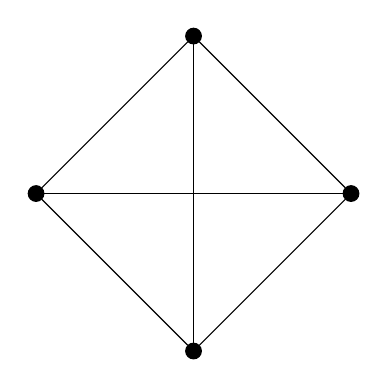
\begin{tikzpicture}[
        every node/.style={circle, draw, fill=black, inner sep=2pt},
        scale=2
    ]
    
    % First TikZ picture
    \node (A) at (0, 1) {};
    \node (B) at (1, 0) {};
    \node (C) at (0, -1) {};
    \node (D) at (-1, 0) {};
    \draw (A) -- (B);
    \draw (A) -- (C);
    \draw (A) -- (D);
    \draw (B) -- (C);
    \draw (B) -- (D);
    \draw (C) -- (D);
    
    \end{tikzpicture}
    n=4
    \end{minipage}
    \hfill
    \begin{minipage}{0.45\textwidth}
    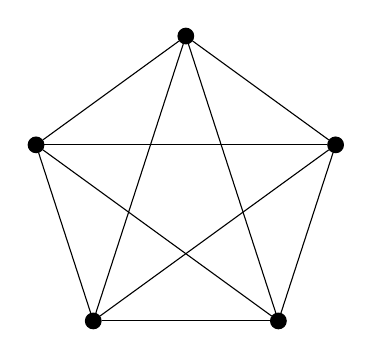
\begin{tikzpicture}[
        every node/.style={circle, draw, fill=black, inner sep=2pt},
        scale=2
    ]
    
    % Second TikZ picture
    \node (A) at (90:1) {};
    \node (B) at (162:1) {};
    \node (C) at (234:1) {};
    \node (D) at (306:1) {};
    \node (E) at (18:1) {};
    \draw (A) -- (B);
    \draw (A) -- (C);
    \draw (A) -- (D);
    \draw (A) -- (E);
    \draw (B) -- (C);
    \draw (B) -- (D);
    \draw (B) -- (E);
    \draw (C) -- (D);
    \draw (C) -- (E);
    \draw (D) -- (E);
    
    \end{tikzpicture}
    n=5
\end{minipage}
The amount of edges is given $\frac{n(n-1)}{2}$

\subsubsection{Bipartite Graphs}
A bipartite graph is a simple graph whose vertices can be divided into 2 disjoint sets U and v such that every edge connect a vertex in U to one in V. It is said to be \textbf{complete} if every vertex in U connects to every vertex in V.

\sbreak

\begin{minipage}{0.45\textwidth}
    \begin{tikzpicture}[
        every node/.style={circle, draw},
        scale=1.5
    ]
    
    % Nodes for bipartite graph
    \node (A1) at (0, 1) {};
    \node (A2) at (0, 0) {};
    \node (A3) at (0, -1) {};
    \node (B1) at (2, 1) {};
    \node (B2) at (2, 0) {};
    \node (B3) at (2, -1) {};
    
    % Edges for bipartite graph
    \draw (A1) -- (B1);
    \draw (A2) -- (B2);
    \draw (A3) -- (B3);
    
    
    \end{tikzpicture}
    
\textbf{Bipartite Graph}
    
\end{minipage}
\hfill
\begin{minipage}{0.45\textwidth}
    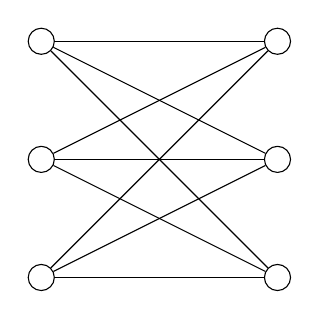
\begin{tikzpicture}[
        every node/.style={circle, draw},
        scale=1.5
    ]
    
    % Nodes for complete bipartite graph
    \node (A1) at (0, 1) {};
    \node (A2) at (0, 0) {};
    \node (A3) at (0, -1) {};
    \node (B1) at (2, 1) {};
    \node (B2) at (2, 0) {};
    \node (B3) at (2, -1) {};
    
    % Edges for complete bipartite graph
    \draw (A1) -- (B1);
    \draw (A1) -- (B2);
    \draw (A1) -- (B3);
    \draw (A2) -- (B1);
    \draw (A2) -- (B2);
    \draw (A2) -- (B3);
    \draw (A3) -- (B1);
    \draw (A3) -- (B2);
    \draw (A3) -- (B3);
    
    % Label
    
    \end{tikzpicture}

\textbf{Complete Bipartite Graph}

Denoted $K_{m,n}$ where m=$|U|$ and n = $|V|$

\end{minipage}
    
\subsubsection{Subgraphs}
G = ($v_s$,$e_s$), and H = ($v$, $e$)

G is said to be a \textbf{subgraph}of H iff $v_s \subseteq v$ and $e_s \subseteq e$

\subsubsection{Degree of Vertex (Undirected)}
The \textbf{degree} of a vertex v, deg(v), is the number of edges incident on v. Edge loops are \underline{counted twice}.

\subsubsection{Total Degree of an Undirected Graph}
The \textbf{total degree} of an undirected graph is the sum of degrees of all its vertices.

\subsubsection{The Handshake Theorem}
G = (V, E)

deg(G) = 2 $\times$ $|E|$

\sub{Corollary 10.1.2}
The total degree of the graph is even.

\sub{Proposition 10.1.3}
There are always an even number of vertices that have odd degree.

\subsubsection{Degree of Vertex (Directed)}
\sub{Indegree}

The indegree of a vertex v, $deg^-(v)$ is the number of directed edges \textbf{pointing towards} v.

\sub{Outdegree}

The outdegree of v, $deg^+(v)$ is the number of edges pointing out \textbf{from} v.

\sub{Total Edges}

$|E|$ = $\sum_{}^{}$ $deg^{-}(v)$ = $\sum_{}^{} deg^+(v)$

\subsubsection{Walks}
A \textbf{walk} is a finite alternating sequence of adjacent vertices and edges of G.
\begin{center}
    $v_0 e_1 v_1 e_2 ... v_{n-1} e_n v_n$
\end{center}

\sub{Trivial Walks}

A walk that is \textbf{trivial} is the walk from v to v consisting of only v.
\begin{center}
    v
\end{center}

\subsubsection{Trails}
A trail from v to w is a walk from v to w that \underline{does not} contain a \textbf{repeated edge}

\subsubsection{Paths}
A path from v to w is a trail that does not contain a repeated vertex.

\subsubsection{Closed Walk}
A closed walk is a walk that starts and ends at the same vertex.

\subsubsection{Circuit}
A circuit is a closed walk of length $\geq 3$ that does not contain a repeated edge.

\subsubsection{Simple Circuit}
A simple circuit is a circuit that does not have any repeated vertex except the first \& last.

\subsubsection{Cyclic}
An undirected graph is \textbf{cyclic} if it contains a loop.

If it doesn't, then it's \textbf{acyclic}

\subsubsection{Connectedness}
Two vertices v and w of a graph G are \textbf{connected} iff there is a walk from v to w.

The \textbf{graph} is connected iff given any two vertices v and w, there is a walk.
\begin{center}
    $\forall v,w \in V,$ $\exists$ a walk from v to w
\end{center}

\sub{Number of edges and vertice in connected graph}
If G=(V,E) is a simple, undirected graph, that is connected, then $|E| \geq |V| - 1$ \theorum{Tutorial 11 Qn 4}

\sub{Minimum bound}
If G is a simple graph with n vertices and every vertex has degree at least floor($\frac{n}{2}$), G is connected

\subsubsection{Circuit removal lemma}
If vertices $v$ and $w$ are a part of a circuit in G and one edge is removed from the circuit, there exists still a trail from v to w in G.

\subsubsection{Connectedness lemma}
If G is connected, then any 2 distinct vertices of G can be connected by a path.

\subsubsection{Circuit removal lemma 2}
If G is connected and G contains a circuit, then an edge of the circuit can be removed and G will still be connected.

\subsubsection{Connected Components}
A graph H is a connected component of a graph G iff:
\begin{enumerate}
    \item The graph H is a \textbf{subgraph} of G.
    \item The graph H is connected
    \item No other connected subgraph of G has H as a subgraph
    \item \begin{enumerate}
        \item Essentially, H is the largest connected subgraph of G.
    \end{enumerate}
\end{enumerate}

\subsubsection{Euler Circuit}
An euler circuit for G is a circuit that contains every vertex and traverses every edge of G exactly \textbf{once}

If a graph contains an Euler Circuit, it is an \textbf{Eulerian graph}

\sbreak

If a graph has an Euler circuit, then every vertex of the graph has a positive even degree. (note that its only one way) \theorum{10.2.2}

Contrapositively, If some vertex of a graph has an odd degree, then the graph does not have an Euler circuit.

\sbreak

If G is \underline{connected} and the degree of every vertex of G is a \underline{even integer}, then G has an Euler circuit. \theorum{10.2.3}

\sbreak

A graph G has an Euler circuit if and only if G is connected and every vertex of G has even degree. \theorum{10.2.4}

\subsubsection{Euler Trail}
An Euler trail from $v$ to $w$ is a sequence of adjacent edges and verteices that starts at v, ends at w, passes thorugh every vertex of G at least once, and traverses every edge of G exactly once.

An Euler Circuit, but it doesn't start and end at the same place.

\sbreak

If G is connected, v and w have odd degree, and all other vertices of G have even degree, then there is a Euler trail from v to w. \theorum{Corollary 10.2.5}

\subsubsection{Hamiltonian Circuit}
A \textbf{Hamiltonian Circuit} for G is a simple circuit that includes every vertex of G.

If a graph has a Hamiltonian Circuit, then it is a Hamiltonian graph.

\subsubsection{Checking for Hamiltonian Circuits}
We can reliably show that a graph does \textcolor{red}{not} have a hamiltonian circuit:

If a graph G has a Hamilotnian circuit, then G has a subgraph H with the following properties:
\begin{enumerate}
    \item H contains every vertex of G.
    \item H is connected.
    \item H has the same number of edges as vertices.
    \item Every vertex of H has degree 2.
\end{enumerate}

\subsubsection{Isomorphic Graphs}
G = ($V_G$, $E_G$) and B = ($V_B$, $E_B$)

G is isomorphic to B, G $\cong$ B iff:
\begin{enumerate}
    \item $\exists$ f: $V_G \rightarrow V_B$ s.t. bijective
    \item $\exists$ h: $E_G \rightarrow E_B$ s.t. bijective
\end{enumerate}
that preserve edge-endpoint functions of G.

That is to say, they are essentially the same graph but represented differently.

\sub{Equivalence Relation of Isomorphism}

Graph isomorphism is an equivalence relation. Find out more what the fak this means.

\subsubsection{Planar Graphs}
A \textbf{planar graph} is a graph that can be drawn without edges crossing

\subsubsection{Kuratowski's theorem}
A finite graph is planar iff it does not contain a subgraph that is a subdivision of the complete graph $K_5$ or the complete bipartite graph $K_{3,3}$. \theorum{Kuratowski}

\sbreak

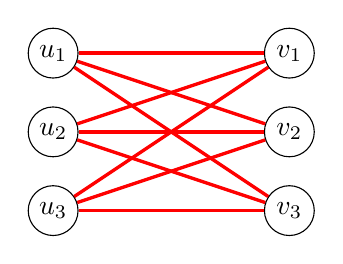
\begin{tikzpicture}[scale=1, auto, node distance=2cm]
    % Define styles
    \tikzstyle{vertex}=[circle, draw, fill=white, inner sep=1pt, minimum size=18pt]
    \tikzstyle{edge} = [draw=black, thick]
    \tikzstyle{highlighted edge} = [draw=red, very thick]

    % Draw the vertices
    \foreach \name/\x/\y in {u_1/0/2, u_2/0/1, u_3/0/0, v_1/3/2, v_2/3/1, v_3/3/0}
        \node[vertex] (\name) at (\x,\y) {$\name$};

    % Draw the edges
    \foreach \u in {u_1,u_2,u_3}
        \foreach \v in {v_1,v_2,v_3}
            \draw[edge] (\u) -- (\v);

    % Highlight edges forming a K_{3,3} subdivision
    % In this case, all edges are part of K_{3,3}
    \foreach \u in {u_1,u_2,u_3}
        \foreach \v in {v_1,v_2,v_3}
            \draw[highlighted edge] (\u) -- (\v);

\end{tikzpicture}



\subsubsection{Euler's Formula}
For a connected planar simple graph G = (V,E), the number of "faces" (regions) = $|E|$ - $|V|$ + 2 \theorum{Euler's Formula}

\sub{Euler's Formula for \#edges in planar graph}

Each face is bounded by at least 3 edges, and each edge shares exactly two faces in a planar graph:
\begin{center}
    $3f \leq 2e \rightarrow f \leq \frac{2e}{3}$
\end{center}

Now, from Euler's formula:
\begin{center}
    $2 + e - v \leq \frac{2e}{3} \rightarrow e \leq 3v - 6$
\end{center}

Thus, for a planar graph the number of edges must satisfy:
\begin{center}
    $e \leq 3v - 6$
\end{center}

For \textbf{bipartite planar graphs}, every face is bounded by at least 4 edges, which means:
\begin{center}
    $e \leq 2v-4$
\end{center}
for planar bipartite graphs

\sub{Using \#edges to determine planarity of Bipartite Graph}

For a planar graph, we have that f + v - e = 2. For a *complete* $K_{m,n}$ graph, number of vertices is given v = m + n. The number of edges is given m*n.

Now if $K_{2,n}$ is planar, the maximum edges it can have must satisfy:
\begin{center}
    $e \leq 2v - 4 \rightarrow 2n \leq 2(2+n) - 4 \rightarrow 2n \leq 2n$
\end{center}
This holds true for any n, so $K_{2,n}$ is planar for any n.

\sub{Proof: Every planar graph has a vertex of degree 5 or less}
Our statement is that Planar $\rightarrow$ $deg(v)\leq 5$

We take the contrapositive, that $\forall v\ deg(v) \geq 6 \rightarrow$ Non planar

\sbreak
\begin{enumerate}
    \item Assume every vertex has a degree of at least 6. This means that there are at least 7 vertices in the graph.
    \item By euler's formula, $e \leq 3v - 6$. This holds because v$\geq$3
    \item By handshake theorem, $\sum deg(v)$ = 2E
    \item By assumption, $\sum deg(v) \geq 6v$
    \item 2E$\geq$6v and thus $E \geq 3v$
    \item However,by euler's formula, $e < 3v- 6$, which is less than $3n$.
    \item As such, euler's formula cannot hold and this graph is nonplanar.
    \item Therefore, the contrpositive is proven
\end{enumerate}

For a graph with degree

\subsubsection{Matrix Representation of Graphs}
We can create an adjancency matrix of an undirected graph by +1'ing in the corresponding rows/cols if there exists edges between the graphs. This is \textbf{symmetric} for a undirected graph

Using this, we can see the number of walks that exist between two vectors.

\sbreak

If G is a graph with vertices $v_1,v_2,...,v_m$ and A is the adjacency matrix of G,then for each positive integer $n$ and for all integers i,j = 1,2,..,m, the $ij$-th entry of $A^n$ is the number of walks of length n from $v_i to v_j$ \theorum{10.3.2}

\sub{Calculating walks}
Note that to calculate walks of length 4, you are taking A * A * A * A
\section{Trees}
\subsection{Definitions}
\subsubsection{Tree}
A simple graph is called \textbf{tree} if and only if it is circuit-free and connected.

\sub{Trivial}

It is trivial if there is only vertex.

\sub{Forest}

If it is not connected, then it is a forest.

\sbreak

Any non-trivial tree has at two vertices of degree 1 \theorum{Lemma 10.5.1}

\sbreak

Any tree with n vertices (n$\geq$1) has n-1 edges.

\sbreak

If G is a connected graph with $n$ vertices and n-1 edges, then G is a tree. \theorum{10.5.4}

\subsubsection{Terminal Vertex (leaf)}
A vertex is a terminal vertex if its degree is \textbf{1}. It is the "end" of that branch of the tree.

\subsubsection{Internal Vertex}
A vertex is internal if its degree is $\geq 2$.

\subsubsection{Rooted Trees}
A \textbf{rooted tree} is a tree in wihch there is one vertex that is distinguished from the others and is called the \textbf{root}.

\sub{Level}

The level of a vertex is the number of edges along the unique path between it and the root

\sub{Height}

The height of the rooted tree is the maximum level of any vertex.

\sub{Child}

The children of a vertex v are all vertices \textbf{adjacent} to v and are 1 level down.


\sub{Parent}

If w is a child of v, v is the parent of w.

\sub{Siblings}

Distinct vertices with the same parent are siblings.

\sub{Ancestor, Descendent.}

Given v \& w, if v lies on the unique path between w and the root, v is the \textbf{ancestor} of w, and w a \textbf{descendent} of v.

\subsection{Binary Trees}
A \textbf{binary tree} is a rooted tree in which every parent has at most two children, left or right.

\sub{Full Binary Tree}

A full binary tree is a binary tree in which each parent has exactly two children

\sbreak

A full binary tree with k internal vertices, has a total of 2k+1 vertices and has k+1 terminal vertices. \theorum{10.6.1}

\sub{Left/Right subtree}

Given any parent v, its left/right subtree is the binary tree whose root is the left/right child of v.

Its vertexes are the descendents of the child, along with the edges.

\sub{Height of Binary Trees}

The height of a binary tree with t terminal vertices has a lower bound:
\begin{center}
    log$_2$t $\leq$ height
\end{center}


\subsubsection{Tree traversal (Depth-First Search)}
There are 3 types of depth-first traversal:
\begin{enumerate}
    \item Pre-Order
    \item \begin{enumerate}
        \item Print data of vertex
        \item Traverse left subtree by recursive call
        \item Traverse right subtree by recursive call
    \end{enumerate}
    \item In-order
    \item \begin{enumerate}
        \item Traverse left subtree by recursive call
        \item Print data of the vertex
        \item Traverse right subtree by recursive call
    \end{enumerate}
    \item Post-order
    \item \begin{enumerate}
        \item Traverse left subtree by recursive call
        \item Traverse right subtree by recursive call
        \item Print data of vertex
    \end{enumerate}
\end{enumerate}

\subsubsection{Spanning Trees}
A spanning tree for a graph G is a subgraph of G that contains every vertex of G and is a tree.

\begin{enumerate}
    \item Every connected graph has a spanning tree
    \item Any 2 spanning tree for a graph have the same number of edges
\end{enumerate}

\subsubsection{Minimum Spanning Tree}
An MST for a weighted graph is a spanning tree which has the least possible total weight compared to all other spanning trees for the graph.

\sub{Kruskal's Algorithm}
\begin{enumerate}
    \item Initialize T to have all vertices of G but no edges
    \item For all edges in graph, sorted from least weight to most weight:
    \item \begin{enumerate}
        \item Check if addition of edge into T introduces a circuit
        \item If it does not, add edge to T.
    \end{enumerate}
\end{enumerate}


\sub{Prim's Algorithm}
\begin{enumerate}
    \item Pick a vertex out of G and initialize T to include this vertex
    \item For all edges incident to the graph T,
    \item \begin{enumerate}
        \item Pick the least weight edge connecting T to a vertex out of T
        \item Add the edge and vertex to T
        \item Repeat
    \end{enumerate}
\end{enumerate}



% TODO: the divider
\pagebreak
\section{Other Theorems}
\subsection[Logical Equivalences]{Logical Equivalences\footnote{2.1.1 pg. 25}}
\begin{table}[ht]
    \centering
    \begin{tabular}{|>{\raggedright}m{4cm}|>{\centering\arraybackslash}m{4cm}|>{\centering\arraybackslash}m{4cm}|}
        \hline
        \textbf{Law} & \textbf{Conjunction (AND)} & \textbf{Disjunction (OR)} \\ \hline
        Commutative laws & \( p \land q = q \land p \) & \( p \lor q = q \lor p \) \\ \hline
        Associative laws & \( p \land q \land r \equiv (p \land q) \land r = p \land (q \land r) \) & \( p \lor q \lor r \equiv (p \lor q) \lor r = p \lor (q \lor r) \) \\ \hline
        Distributive laws & \( p \land (q \lor r) \equiv (p \land q) \lor (p \land r) \) & \( p \lor (q \land r) \equiv (p \lor q) \land (p \lor r) \) \\ \hline
        Identity laws & \( p \land \text{true} = p \) & \( p \lor \text{false} = p \) \\ \hline
        Negation laws & \( p \land \sim p = \text{false} \) & \( p \lor \sim p = \text{true} \) \\ \hline
        Double negative law & \( \sim(\sim p) = p \) &  \\ \hline
        Idempotent laws & \( p \land p = p \) & \( p \lor p = p \) \\ \hline
        Universal bound laws & \( p \lor \text{true} = \text{true} \) & \( p \land \text{false} = \text{false} \) \\ \hline
        De Morgan’s laws & \( \sim(p \land q) \equiv \sim p \lor \sim q \) & \( \sim(p \lor q) \equiv \sim p \land \sim q \) \\ \hline
        Absorption laws & \( p \lor (p \land q) \equiv p \) & \( p \land (p \lor q) \equiv p \) \\ \hline
        Negation of true and false & \( \sim \text{true} \equiv \text{false} \) & \( \sim \text{false} \equiv \text{true} \) \\ \hline
    \end{tabular}
\end{table}

\vspace{10pt}

\textbf{Advanced Logical Statements}

Note that if there is a lot of fluff on screen, you can still apply basic laws.

e.g. $(p \wedge q \wedge s) \vee (!p \wedge q \wedge !r \wedge t) \vee q \vee (q \wedge r \wedge s \wedge !t)$

To do advanced logical statements, try to look for common elements, then apply basic rules.

If you localise the last term and let some random variable $z = r \wedge s \wedge$\negation t, then we can easily see the absorption law: $q \vee (q \wedge z)$. Be resourceful.

Additionally, think of counterexamples. Any situation in which it's possible for an implication to have a T $\rightarrow$ F value invalidates the logical statement.

\subsection[Every integer is a rational number]{Every integer is a rational number\footnote{4.2.1 pg. 19}}

\subsection[The sum of any two rational numbers is rational]{The sum of any two rational numbers is rational\footnote{4.2.2 pg. 20}}

\subsection[Positive Divisor of a Positive Integer]{Positive Divisor of a Positive Integer\footnote{4.3.1 pg. 25}}
For all positive integers a and b, if a $\mid$ b, then a $\leq$ b

\subsection[Divisors of 1]{Divisors of 1\footnote{4.4.2 pg. 25}}
The only divisors of 1 are 1 and -1.

\subsection[Transitivity of Divisibility]{Transitivity of Divisibility\footnote{4.3.3 pg.27}}
For all integers a,b, and c, if $a\mid b, b\mid c, \rightarrow a\mid c$

\subsection[There is no greatest integer]{There is no greatest integer\footnote{4.7.1 pg.29}}

\subsection[Evenness of $n^2$]{Evenness of $n^2$   \footnote{4.6.4 pg.32}}
For all integers n, if $n^2$ is even, then n is even.

\subsection[Oddness of $n^2$]{Oddness of $n^2$   \footnote{Tutorial 1, Qn. 11}}
If n is an integer, $n^2$ is odd $/iff$ n is odd.

\subsection{Quotient-Remainder Theorum}
Given any integer n and positive integer d, there exist unique integers q and r such that

$n = dq + r$ and $0\leq r < d$

\subsection[The product of any two odd integers is an odd integer]{The product of any two odd integers is an odd integer \footnote{Tutorial 1, Qn. 10}}

\section{Random Definitions}
\subsection{Congruence}
Let $a,b \in \mathbb{Z}^+.$ Then, a is \textbf{congruent} to b modulo n iff a-b = nk for some k $\in \mathbb{Z}$. In other words, n $\mid$(a-b).

Written as $a\equiv b (mod\ n)$

Congruence-mod n is an equivalence relation on $\mathbb{Z}$ for every n $\in \mathbb{Z}^+$

\subsubsection{Congruence Modulo Quotient}
Recall dividing by equivalence relation.

The quotient $\mathbb{Z} /\sim_\textbf{x}$ where $\sim_\textbf{x}$ is the congruence-modulo-\textbf{x} relation on Z, is denoted $Z_\textbf{x}$

Essentially, it is all the partitions of congruence modulo on some integer x.

\sub{Addition and multiplication on the quotient}
[x] + [y] = [x+y]
(the quotient of x + quotient of y is simply quotient of x+y; congruence modulo x+y)

\sbreak

[x] * [y] = [x*y]

\subsection{Recurrence Relations}
A \textbf{recurrence relation} of a sequence is aformula that relates each term to some predecessor(s). Fibonnaci Sequence is an example.

\section{Methods of Proofing}
\subsection{Constructive Proof of Existential Statements}
Given a statement
\begin{center}
    $\exists x \in D Q(x)$
\end{center}
We can prove it by using one of the \textcolor{blue}{constructive proofs of existence}:
\begin{enumerate}
    \item Find an $x$ in D that makes Q(x) true
    \item Give a set of directions for finding such an x
\end{enumerate}


\subsection{Vertex colouring}
Is an assignment of colours to vertices that no two adjacent vertices have the same colour.

\sub{Four-colour conjecture}
You can accomplish a vertex colouring of any graph using 4 colours.


\subsection{Disproving Universal statements by Counterexample}
Given a universal conditional:
\begin{center}
    $\forall x \in D\ (P(x)\rightarrow Q(x))$
\end{center}
We can show that this statement is \textcolor{red}{false} by showing that \textcolor{red}{its negation is true}
\begin{center}
    $\exists x \in D\ (P(x)\wedge \text{\negation} Q(x))$
\end{center}

\subsection{Proof by exhaustion}
Given a universal conditional:
\begin{center}
    $\forall x \in D\ (P(x)\rightarrow Q(x))$
\end{center}
Showing that this statement is true for \textbf{all} of D shows that the statement is true.

\subsection{Generalizing from the generic particular}
Showing that every element of a set satisfies a certain property, suppose x is \textcolor{red}{particular} but \textcolor{red}{arbitrarily}chosen element of the set, and show that x satisfies the property.

e.g.
If $m$ and $n$ are two particular but arbitrarily chosen integers, m = 2r and n = 2s. Using this, prove the wanted property.

\subsection{Division into cases}
If the proof has multiple cases, e.g. even and odd, we split the proof into cases and solve each one individually

\subsubsection{Without Loss of Generality}
WLOG are when the proof has multiple cases, but the proof of one case is exactly the same as the proof of the other case. As such, we can use WLOG to generalize the proof. \footnote{Assignment 1 Qn. 5}


\subsection{Proof By Contradiction}
\begin{enumerate}
    \item Suppose that the statement to be proved, S, is \textcolor{red}{false}. So, \negation S is \textcolor{blue}{true}
    \item Show that this supposition leads logically to a Contradiction
    \item Conclude that the statement S is true.
\end{enumerate}

There's no need to \textcolor{red}{negate the premise}!

\vspace{10pt}

Another example, suppose we know or have an intuition that a property is true. Let's say if $g\circ f$ is injective, then f is injective. If we want to proof that f is injective, we can assume that f is \textit{not} injective. Then, do the proof as usual, and once there's a contradiction we know that the assumption is false.

\subsection{Proof by Contraposition}
Recall that a contraposition is $\equiv$ the original statement. Proving a contraposition is true is equivalent to proving that the original statement is true.

\begin{enumerate}
    \item Suppose the statement to be proved is $\forall x \in D\ (P(x)\rightarrow Q(x))$
    \item Rewrite the statement into Contrapositive form:
    \begin{center}
        $\forall x \in D\ (\text{\negation}Q(x)\rightarrow \text{\negation}P(x))$
    \end{center}
    \item Prove the contrapositive directly
    \item Therefore, the original statement is true.
\end{enumerate}

\end{document}